\chapter{Motivation and Background of \smt} \label{sec:smt-motivation}

\section{Why Are Multithreaded Programs So Hard to Get Right?} \label{sec:why}

\begin{figure*}[t]
\begin{center}
\subfloat[{\em Traditional.}]{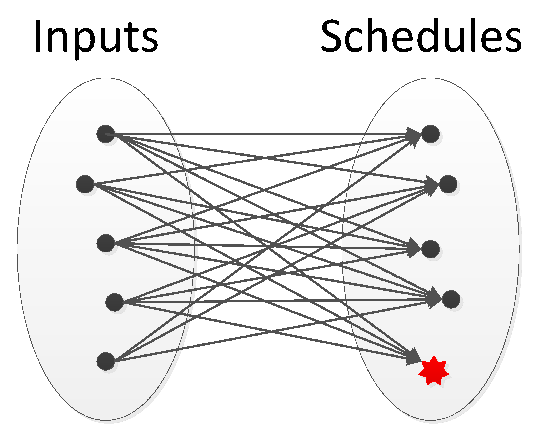
\includegraphics[width=.23\linewidth]{figures/nondet}\label{fig:nondet}}
\subfloat[{\em Deterministic.}]{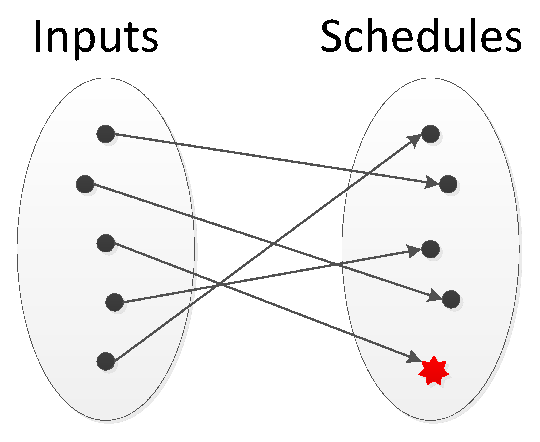
\includegraphics[width=.23\linewidth]{figures/dmt}\label{fig:dmt}}
\subfloat[{\em Stable (deterministic).}]{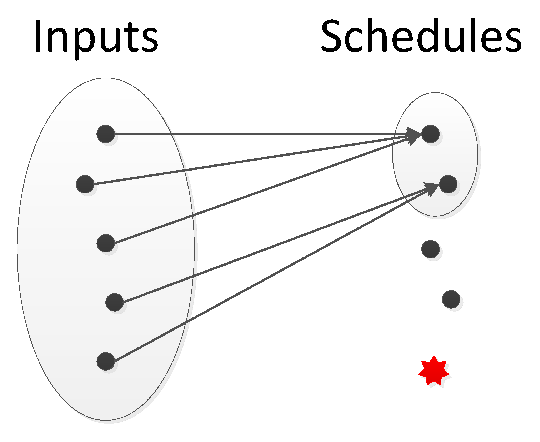
\includegraphics[width=.23\linewidth]{figures/smt}\label{fig:smt}}
\subfloat[{\em Stable (nondeterministic).}]{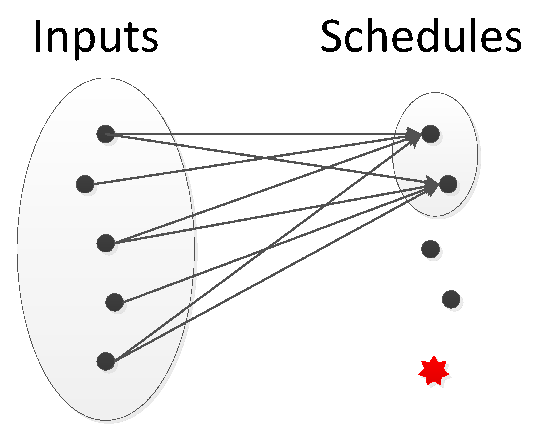
\includegraphics[width=.23\linewidth]{figures/smtn}\label{fig:smtn}}
\vspace{-.05in}
\caption{Different multithreading approaches. Red stars represent buggy
  schedules.  Traditional multithreading (\subref*{fig:nondet})
  is a conceptual many-to-many mapping where one input may execute under
  many schedules because of nondeterminism, and many inputs may execute
  under one schedule because a schedule fixes the order of the
  communication operations but allows the local computations to operate on
  any input data.  DMT (\subref*{fig:dmt}) may
  map each input to an arbitrary schedule, reducing programs' robustness
  on input perturbations.  \smt (\subref*{fig:smt} and
  \subref*{fig:smtn}) reduces the total set of schedules for all inputs (represented by the shrunk ellipses),
  increasing robustness and improving reliability.
  \smt and DMT are orthogonal: a \smt system can be deterministic
  (\subref*{fig:smt}) or nondeterministic (\subref*{fig:smtn}).}
\vspace{-.2in}
\end{center}
\end{figure*}

We start with preliminaries, then describe the challenges caused by
nondeterminism and by too many schedules.  We then explain why
nondeterminism is a lesser cause than too many schedules.

\subsection{Preliminaries: Inputs, Schedules, and Buggy Schedules}

To ease discussion, we use \emph{input} to broadly refer to the data a
program reads from its execution environment, including not only the data
read from files and sockets, but also command line arguments, return
values of external functions such as \v{gettimeofday}, and any external data that can affect program
execution.  We use \emph{schedule} to broadly refer to the (partially or
totally) ordered set of communication operations in a multithreaded
execution, including synchronizations (\eg, \v{lock} and
\v{unlock} operations) and shared memory accesses (\eg, \v{load} and
\v{store} instructions to shared memory). Of all the schedules, most run
fine, but some trigger concurrency errors, causing program crashes,
incorrect computations, deadlocked executions, and other failures.
Consider the toy program below: \lgrindfile{code/sync-bug.cpp}
\noindent The schedule in which thread 2 gets the lock before thread 1
causes a dereference-of-NULL failure.  Consider another example.  The toy program
below has data races on \v{balance}: \lgrindfile{code/race-bug.cpp}
\noindent 
The schedule with the statements executed in the order shown corrupts
\v{balance}. We call the schedules that trigger concurrency errors
\emph{buggy schedules}.  Strictly speaking, the errors are in the
programs, triggered by a combination of inputs and schedules.  However,
typical concurrency errors, such as most errors appeared in previous
studies~\cite{lu:concurrency-bugs,con:hotpar12}, depend much more on the
schedules than the inputs (\eg, once the schedule is fixed, the bug
occurs for all inputs allowed by the schedule).  Thus, recent research on
testing multithreaded programs (\eg,~\cite{musuvathi:chess:osdi08}) is
focused on effectively testing schedules to find the buggy ones.

\subsection{Challenges Caused by Nondeterminism} \label{sec:nondet}

%% Determinism requires that executions of the same program on the same input
%% (as defined in the previous subsection) always yield the same behavior.
%% Nondeterminism, the opposite of determinism, requires that these
%% executions yield different behaviors.  
A multithreaded program is nondeterministic because even with the same
program and input, different schedules may still lead to different
behaviors.  For instance, the two toy programs in the previous subsection
do not always run into the bugs.  Except for the schedules described, the
other schedules lead to correct executions.

This nondeterminism raises many challenges, especially in
testing and debugging.  Suppose an input can execute under $n$ schedules.
Testing $n-1$ schedules is not enough for complete reliability because the
single untested schedule may still be buggy.  An execution in the field
may hit this untested schedule and fail.  Debugging is challenging, too.
To reproduce a field failure for diagnosis, the exact input alone is not
enough. Developers must also manage to reconstruct the buggy schedule out
of $n$ possibilities.

Figure~\ref{fig:nondet} depicts the traditional multithreading approach.
Conceptually, it is a many-to-many mapping, where one input may execute
under many schedules because of nondeterminism, and many inputs may
execute under one schedule because a schedule fixes the order of the
communication operations but allows the local computations to operate on
any input data.

\subsection{Challenges Caused by Too Many Schedules}

%% We believe most challenges in making reliable multithreaded programs has a
%% rather quantitative root cause: these programs have too many schedules.
%% To make a multithreaded program completely reliable, we must ensure that
%% no schedules are buggy, either manually by thinking really hard or
%% automatically by applying tools.  Either way, the number of the schedules
%% determines the amount of efforts and resources needed.

% Unfortunately, a 
A typical multithreaded program has an enormous number of schedules.  For
a single input, the number of schedules is asymptotically exponential in
the schedule length.  For instance, given $m$ threads each competing for a
lock $k$ times, each order of lock acquisitions forms a
schedule,
%\footnote{A lock implementation that grants locks to threads
%  based on the arrival order, such as a ticket lock, does not reduce the
%  set of schedules, because the threads may \emph{arrive} at the lock
%  operations in different orders.}
easily yielding $\frac{(mk)!}{(k!)^m} \ge
(m!)^k$ total schedules---a number exponential in both $m$ and $k$.
%If each thread acquires the lock $k$ times, the number of schedules becomes $\frac{(nk)!}{k!} \ge (n!)^k$, exponential in both $n$ and $k$.
Aggregated over all inputs, the number of schedules is even greater.

%% implementation that grants
%% threads the lock in the order in which they arrive at the lock operations,
%% such as a ticket lock, 

Finding a few buggy schedules in these exponentially many schedules raises
a series of ``needle-in-a-haystack'' challenges.  For instance, to write
correct multithreaded programs, developers must carefully synchronize
their code to weed out the buggy schedules.  As usual, humans err when
they must scrutinize many possibilities to locate corner cases. Various
forms of testing tools suffer, too.  Stress testing is the common method
for (indirectly) testing schedules, but it often redundantly tests the
same schedules while missing others.  Recent tools
(\eg,~\cite{musuvathi:chess:osdi08}) systematically test
schedules for bugs, but we seriously lack resources to cover more than a tiny
fraction of all exponentially many schedules.
%% Static bug detectors, which check code without running it,
%% over-approximate these schedules, so they often emit many false bug
%% reports.
% analyzing: Nall static dynamic

\subsection{Determinism Is Not As Useful as Commonly Perceived}

To address the challenges raised by nondeterminism, researchers including
us have dedicated much effort and built several systems that force a
multithreaded program to always run the same schedule on the same input,
bringing determinism to multithreading.  This determinism does have value
for reliability.  For instance, one testing execution now validates all
future executions on the same input.  Reproducing a concurrency error now
requires only the input.

In contrast to this effort, little has been done to solve the
challenges caused by too many schedules.  We believe
the community has charged nondeterminism more than its share of the guilt
and overlooked the main culprit---a rather quantitative cause that
multithreaded programs simply have too many schedules.
We argue that, although determinism has value, its value
is smaller than commonly perceived.  It is neither sufficient nor
necessary for reliability.

%% Researchers have built several systems to make multithreading
%% deterministic, hoping to address the challenges raised by nondeterminism.
%% Yet, little has been done to solve the needle-in-a-haystack challenges
%% caused by too many schedules.  We believe the community has charged
%% nondeterminism more than its share of the guilt and overlooked the main
%% culprit that multithreaded programs simply have too many
%% schedules.  We argue that determinism, the cure of
%% nondeterminism, is neither sufficient nor necessary for reliability.

\para{Determinism $\centernot \implies$ reliability.} Determinism is a
narrow property: same input + same program = same behavior. It has no
jurisdiction if the input or program changes however slightly.  Yet, we
often expect a program to be robust or stable against slight program
changes or input perturbations.  For instance, adding a debug \v{printf}
should in principle not make the bug
disappear.  Similarly, a single bit flip of a file should usually not
cause a compression utility to crash. Unfortunately, determinism
does not provide this stability and, if na\"{i}vely implemented,
even undermines it.

To illustrate, consider the system depicted in
Figure~\ref{fig:dmt} which maps each input to an arbitrary schedule. This
mapping is perfectly deterministic, but it destabilizes program
behaviors on multiple inputs.  A single bit flip may force a program to
discard a correct schedule and adventure into a vastly different, buggy
schedule.

This instability is counterintuitive at least,
and raises new reliability challenges.  For instance, testing one input
provides little assurance on very similar inputs, despite that the differences
in input do not invalidate the tested schedule.  Debugging now requires
every bit of the bug-inducing input, including not only the data a user
typed, but also environment variables, shared libraries, \etc.  A
different user name?  Error report doesn't include credit card numbers?
The bug may never be reproduced, regardless of how many times developers
retry, because the schedule chosen by the deterministic system for the
altered input happens to be correct.  Note that even a correct
sequential program may show very different behaviors for small input
changes across boundary conditions, but these conditions are typically
infrequent and the different behaviors are intended by developers.  In
contrast, the instability introduced by the system in Figure~\ref{fig:dmt}
is artificial and on all inputs.

Besides inputs, na\"{i}vely implemented determinism can destabilize
program behaviors on minor code changes, so adding a debug \v{printf}
causes the bug to deterministically disappear.  Another problem is that
the number of all possible schedules remains enormous, so the coverage of
schedule testing tools remains low.

In practice, to mitigate these problems, researchers have to augment
determinism with other techniques.  To support debug \v{printf}, some
propose to temporarily revert to nondeterministic
execution~\cite{dmp:asplos09}.  DMP~\cite{dmp:asplos09},
CoreDet~\cite{coredet:asplos10}, and Kendo~\cite{kendo:asplos09} change
schedules only if the inputs change low-level instructions executed.
Although better than mapping each input to an arbitrary schedule, they
still allow small input perturbations to destabilize schedules
unnecessarily when the perturbations change the low-level instructions
executed (\eg, one extra \v{load} executed), observed in our
experiments~\cite{cui:tern:osdi10}. Our \tern, \peregrine, and \parrot systems and others'
\dthreads~\cite{dthreads:sosp11} built subsequently to \tern combine DMT
with \smt (elaborated next section) to frequently reuse schedules on a
wide range of inputs for stability.

% These systems

%% For those curious minds, deterministic multithreading systems may be implemented in
%% several ways.  A frequent scheme is to schedule threads based on
%% \emph{logical clocks}~\cite{coredet:asplos10,kendo:asplos09}, instead of
%% physical clocks which change nondeterministically across executions.
%% Specifically, each thread maintains a logical clock that ticks based on
%% the code the thread has run.  For instance, if a thread has completed 50
%% \v{load} instructions, tick its clock by 50.  Moreover, threads
%% communicate only when their logical clocks have deterministic values (\eg,
%% the smallest across the logical clocks of all
%% threads~\cite{kendo:asplos09}).  In short, local executions tick logical
%% clocks deterministically, and logical clocks force threads to communicate
%% deterministically.  By induction, a multithreaded execution becomes
%% deterministic.  It is straightforward to see that a slight input change or
%% an additional \v{printf} statement may change the number of completed load
%% instructions, thus altering the schedule and destabilizing program
%% behaviors.

\para{Reliability $\centernot \implies$ determinism.} Determinism
is a binary property: if
an input maps to $n > 1$ schedules, executions on this input may be
nondeterministic, however small $n$ is.  Yet, a nondeterministic system
with a small set of total schedules can be made reliable easily.  Consider an
extreme case, the nondeterministic system depicted in
Figure~\ref{fig:smtn} which maps all inputs to at most two schedules.  In this
system, the challenges caused by nondeterminism (\S\ref{sec:nondet}) are
easy to solve.  For instance, to reproduce a field failure given an input,
developers can easily afford to search for one out of only two schedules.
To offer an analogy, a coin toss is nondeterministic, but humans have
no problem understanding and doing it because there are only two possible
outcomes.

%% Unfortunately, DMT alone may not reduce the set of all possible schedules.
%% It eliminates nondeterminism, but nondeterminism is only a derived problem
%% caused by the exponentially many schedules projected on an individual
%% input.  A legal DMT system can still map an input to an arbitrary
%% schedule, as depicted in Figure~\ref{fig:dmt}.  The set of DMT schedules
%% thus remains
%% % Since the set of inputs is also enormous
%% enormous---asymptotically as enormous as the set of schedules allowed by
%% traditional multithreading.  Consequently, multithreaded programs with DMT
%% remain difficult to write, test, analyze, \etc.  For instance, testing all
%% schedules remains hard, because it requires testing all inputs.  

%% Consider a loose, non-tech analogy.  A multithreaded execution is like a
%% group of cars driving down parallel lanes, where the group of cars is the
%% input and are the sequence of lane changes (``lane-change plan'') is the
%% schedule.  A buggy schedule causes a program to misbehave, like an unsafe
%% lane-change plan causing cars to collide.  With DMT, although each group
%% of cars sticks to one lane-change plan, given enough groups of cars and an
%% arbitrary plan for each group, some group will eventually collide.

%% An arbitrary mapping as Figure~\ref{fig:dmt} also destabilizes program
%% behaviors over multiple inputs: a slight input change, as slight as a bit
%% flip, may force a program to discard a correct schedule and (ad)venture
%% into a vastly different, buggy schedule.  This instability is
%% counterintuitive at least, and actually creates new reliability
%% challenges. For instance, testing one input provides little confidence on
%% very similar inputs.  Debugging now may require every bit of the
%% bug-inducing input, including not only the data a user typed, but also
%% environment variables, shared libraries, \etc.  A different user name?
%% Error report doesn't include credit card numbers?  The bug may never be
%% reproduced, regardless of how many times developers retry, because the
%% schedule chosen by DMT for the altered input happens to be correct.

%% We believe the intermingle of two factors has largely contributed to the
%% difficulty in getting correct multithreaded programs.  First, a typical
%% multithreaded program has an enormous---asymptotically exponential in the
%% schedule lengths---number of schedules.  For instance, given $n$ threads
%% competing for a lock, each order of lock acquisitions forms a schedule,
%% easily yielding $n!$ total schedules.

%% Second, of the exponentially many schedules, most are correct, but some
%% trigger programming bugs and cause the program to crash, deadlock, compute
%% an incorrect result, or misbehave in other ways.  For example, the toy
%% program below has a dereference-of-NULL bug involving two threads:
%% \lgrindfile{code/sync-bug.cpp}
%% \noindent If thread 2 gets the lock before thread 1, the bug is triggered.
%% The toy program below has data races on \v{balance}:
%% \lgrindfile{code/race-bug.cpp}
%% \noindent The schedule shown corrupts \v{balance}.

%% A \emph{buggy schedule} is one where the threads mis-communicate, causing
%% a bad behavior, such as a program crash, a deadlock, or an incorrect
%% output.  For example, the toy program below has two schedules due to
%% nondeterminism in locking: \lgrindfile{code/sync-bug.cpp}
%% \noindent The schedule with thread 1 getting the lock first is correct,
%% while the other one leads to a dereference-of-NULL crash.  The toy program
%% below also has two schedules due to nondeterminism in data races where two
%% threads access the same shared memory location and at least one access is
%% w rite \lgrindfile{code/race-bug.cpp}
%% \noindent The schedule with thread 1 writing variable \v{result} first is
%% correct, while the other one prints out an incomplete \v{result}.

%% Although the two toy programs are based on real-world bugs in popular
%% multithreaded programs, we have greatly simplified them to highlight the
%% buggy schedules.  In reality, 

%% The combination of these two factors turns reliable parallelism into a
%% needle-in-a-haystack problem, causing many reliability challenges.  For
%% instance, to write correct multithreaded programs, developers must
%% carefully synchronize their code to weed out the buggy schedules.  As
%% usual, humans err when they must scrutinize many possibilities to locate
%% corner cases.  Various forms of testing tools suffer, too.  They require
%% running programs, but we just don't have the time and resources to run
%% more than a tiny fraction of all possible schedules, and the next
%% execution may well hit an untested schedule containing bugs.

%% Static (compile-time) analysis over all schedules must over-approximate
%% all schedules into something enumerable at compile time, resulting in poor
%% precision and many false error reports.  

%% \begin{figure}[t]
%% \centering
%% 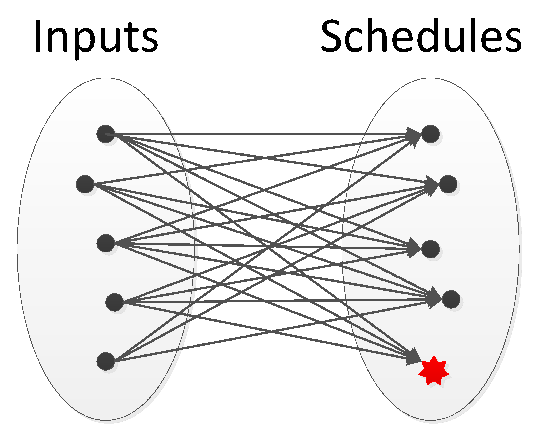
\includegraphics[width=.5\linewidth]{figures/nondet}
%% \caption{{\em Traditional multithreading.} The red star represents a buggy
%%   schedule. } \label{fig:nondet}
%% \end{figure}

%% \begin{figure*}[t]
%% \centering
%% \begin{tabular}{cccc}
%% \parbox{.22\textwidth}{
%% \centering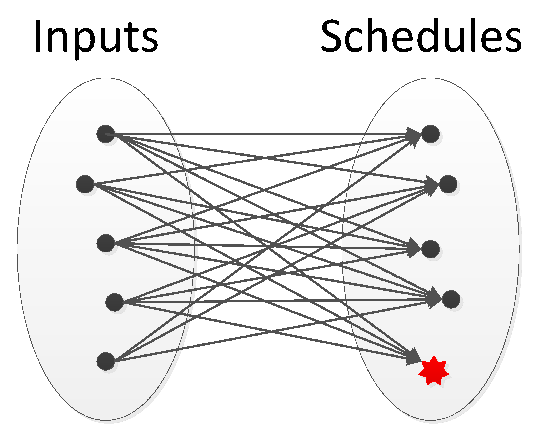
\includegraphics[width=\linewidth]{figures/nondet}} &
%% \parbox{.22\textwidth}{
%% \centering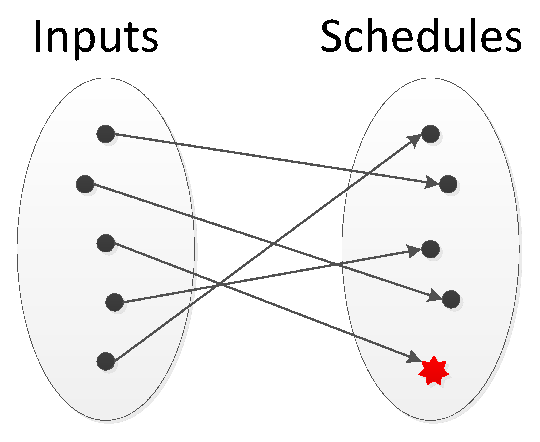
\includegraphics[width=\linewidth]{figures/dmt}} &
%% \parbox{.22\textwidth}{
%% \centering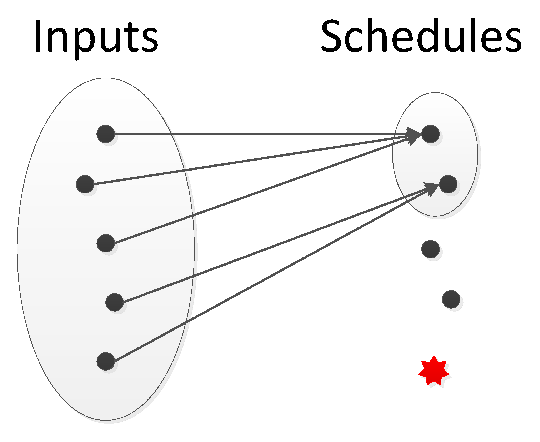
\includegraphics[width=\linewidth]{figures/smt}} &
%% \parbox{.22\textwidth}{
%% \centering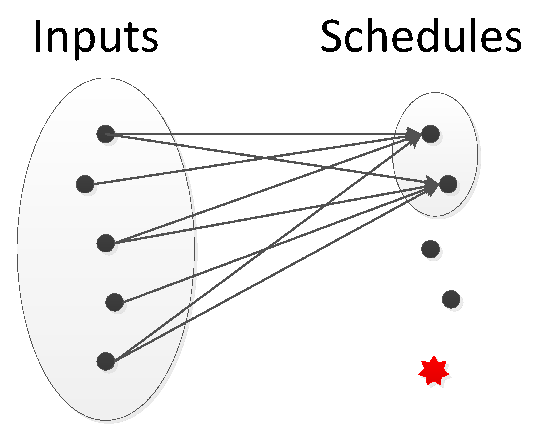
\includegraphics[width=\linewidth]{figures/smtn}} \\
%% \parbox{.22\textwidth}{
%% \centering\caption{{\em Traditional multithreading.} The red star represents a buggy
%%   schedule. } \label{fig:nondet}} &
%% \parbox{.22\textwidth}{
%% \centering\caption{\em Deterministic multithreading.} \label{fig:dmt}} &
%% \parbox{.22\textwidth}{
%% \centering\caption{\em Stable (deterministic) multithreading.} \label{fig:smt}} &
%% \parbox{.22\textwidth}{
%% \centering\caption{\em Stable (nondeterministic) multithreading.} \label{fig:smt}} \\
%% \end{tabular}
%% \end{figure*}

%% For any given input, the number of schedules that can process the input
%% may also be large, and these schedules may again mix correct and buggy
%% schedules.  This mix makes today's multithreading systems
%% \emph{nondeterministic}:
% makes it hard to understand, test, and debug multithreaded programs.  

%% The enormous, skewed mix of schedules, projected onto an individual input,
%% causes the problem of \emph{nondeterminism}: repeated executions of a
%% multithreaded program on the input may lead to different (\eg, correct
%% \vs buggy) behaviors, depending on which schedule is run.  Nondeterminism
%% also creates many reliability challenges, though these challenges concern
%% each individual input.  For instance, testing becomes less effective: a
%% program may run correctly on an input in the testing lab because the
%% schedules tested happen to be correct, but executions on the same exact
%% input may still fail in the field when the program hits a buggy schedule.
%% Debugging is extremely challenging, too: to reproduce such a ``wild'' bug
%% on a developer machine, the exact input alone is not enough; developers
%% must also manage to reconstruct a buggy schedule out of many possible
%% schedules.

% a schedule fixes only the communication operations, but it allows flexible local computations

%% Conceptually, nondeterministic multithreading forms a one-to-many mapping
%% from inputs to schedules, illustrated in

% \section{Deterministic Multithreading} \label{sec:dmt}

%% \begin{figure}[t]
%% \centering
%% 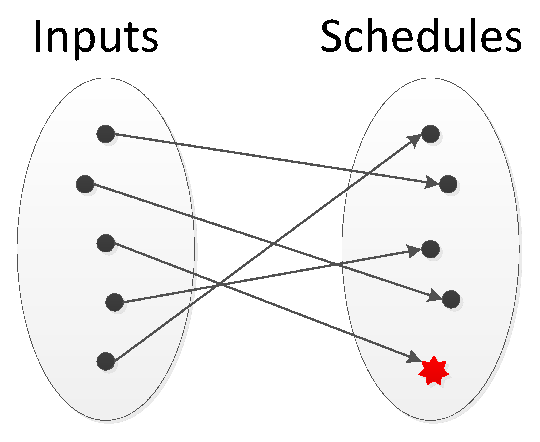
\includegraphics[width=.5\linewidth]{figures/dmt}
%% \caption{\em Deterministic multithreading.} \label{fig:dmt}
%% \end{figure}

%% Several groups of researchers have attributed the multithreaded
%% programming difficulty largely to
%% nondeterminism~\cite{lee06,dmp:asplos09,grace:oopsla09,dpj:oopsla09}. To battle
%% nondeterminism, some have pioneered \emph{deterministic multithreading
%%   (DMT)} systems that force a multithreaded program to always use the same
%% schedule on the same input.  Figure~\ref{fig:dmt} depicts a conceptual DMT
%% mapping from inputs to schedules.

% On the surface, DMT appears to be the cure for multithreaded programs.
%% DMT may be implemented in several ways.  A common scheme is to schedule
%% threads based on \emph{logical
%%   clocks}~\cite{coredet:asplos10,kendo:asplos09}, instead of physical
%% clocks which change nondeterministically across executions.
%% Specifically, each thread maintains a logical clock that ticks
%% based on the code the thread has run.  For instance, if a thread has
%% completed 50 \v{load} instructions, tick its clock by 50.  Moreover,
%% threads communicate only when their logical clocks have deterministic
%% values (\eg, the smallest across the logical clocks of all
%% threads~\cite{kendo:asplos09}).  In short, local executions tick logical
%% clocks deterministically, and logical clocks force threads to communicate
%% deterministically.  By induction, a multithreaded execution becomes
%% deterministic.

%% By eliminating nondeterminism, DMT solves the reliability challenges on
%% each individual input.  For instance, it makes testing more effective
%% because one test execution on an input suffices to test this input's only
%% schedule.  Debugging becomes easier, too, because the exact input suffices
%% to reproduce a bug: DMT automatically reconstructs the buggy schedule for
%% the developers.

%% DMT alone leaves many
%% reliability challenges open.
%% this set is as
%% large as the set of schedules allowed by nondeterministic multithreading.

%% Unfortunately, DMT alone may not reduce the set of all possible schedules.
%% It eliminates nondeterminism, but nondeterminism is only a derived problem
%% caused by the exponentially many schedules projected on an individual
%% input.  A legal DMT system can still map an input to an arbitrary
%% schedule, as depicted in Figure~\ref{fig:dmt}.  The set of DMT schedules
%% thus remains
%% % Since the set of inputs is also enormous
%% enormous---asymptotically as enormous as the set of schedules allowed by
%% traditional multithreading.  Consequently, multithreaded programs with DMT
%% remain difficult to write, test, analyze, \etc.  For instance, testing all
%% schedules remains hard, because it requires testing all inputs.  

%% Consider a loose, non-tech analogy: a multithreaded execution is like cars driving
%% down parallel lanes, where the sequence of lane changes (``lane-change
%% plan'') is the schedule.  A buggy schedule causes a program to misbehave,
%% like an unsafe lane-change plan causing cars to collide.  With DMT,
%% although each group of cars sticks to one lane-change plan, given enough
%% groups of cars and an arbitrary plan for each group, some group will
%% eventually collide.

% yet we just cannot test all groups of cars.
%% To ease understanding, we liken a multithreaded execution to a group of
%% cars driving down parallel lanes of a highway, where the cars are the
%% input and the sequence of lane changes (``lane-change plan'') is the
%% schedule.  We will refer to this non-technical analogy later in the
%% article.


%% like unsafe lane-change plans cause cars to collide.

%% is like the same group of cars taking a random lane-change plan each time
%% they drive down a highway.  It 


%% Referring
%% back to our non-technical analogy: although each group of cars sticks to
%% one lane-change plan, given enough groups of cars and an arbitrary plan
%% for each group, some group will eventually collide, yet we just cannot
%% test all groups of cars.

%% Thus, even with DMT, it remains difficult to understand, test, and analyze
%% multithreaded programs.  A non-tech analogy: the execution of a
%% multithreaded program is like a group of cars driving down parallel lanes
%% of a highway, where cars are the input and their lane-change plan is the
%% schedule.  In nondeterministic multithreading, cars choose a different
%% lane-change plan each time they pass the highway, and sometimes they
%% collide and cause the program to crash.  In deterministic multithreading,
%% each group of cars fixes their lane-change plan, bug given enough cars and
%% arbitrary plans, some cars will also collide and cause the program to
%% crash.

%% An arbitrary mapping as Figure~\ref{fig:dmt} also destabilizes
%% program behaviors over multiple inputs: a slight input change, as slight
%% as a bit flip, may force a program to discard a correct schedule and
%% (ad)venture into a vastly different, buggy schedule.  This instability is
%% counterintuitive at least, and actually creates new reliability
%% challenges. For instance, testing one input provides little confidence on very
%% similar inputs.  Debugging now may require every bit of the bug-inducing
%% input, including not only the data a user typed, but also environment
%% variables, shared libraries, \etc.  A different user name?  Error report
%% doesn't include credit card numbers?  The bug may never be reproduced,
%% regardless of how many times developers retry, because the schedule
%% chosen by DMT for the altered input happens to be correct.
% DMT forces a different schedule.

%% unstable over inputs: discard a correct schedule, ad into.

%% although DMT solves challenges on each isolated input, it
%% alone leaves many reliability challenges open because it ignores the
%% aggregated program behaviors over multiple inputs.  

%% A legal DMT system may
%% map an input to an arbitrary schedule, like the one shown in
%% Figure~\ref{fig:dmt}.  Other examples include DMT systems that, for load
%% balancing, tick their logical clocks based on low-level
%% instructions~\cite{coredet:asplos10,kendo:asplos09}.  Arbitrary mappings
%% actually defeat the benefits of determinism by causing at least two
%% issues:

%% First, the set of the DMT-mapped schedules is still enormous.
%% Asymptotically, this set is as large as the set of schedules allowed by
%% nondeterministic multithreading.  Thus, even with DMT, it remains
%% difficult to understand, test, and analyze multithreaded programs.  A
%% non-tech analogy: the execution of a multithreaded program is like a group
%% of cars driving down parallel lanes of a highway, where cars are the input
%% and their lane-change plan is the schedule.  In nondeterministic
%% multithreading, cars choose a different lane-change plan each time they
%% pass the highway, and sometimes they collide and cause the program to
%% crash.  In deterministic multithreading, each group of cars fixes their
%% lane-change plan, bug given enough cars and arbitrary plans, some cars
%% will also collide and cause the program to crash.

%% Second, although DMT enforces the same schedule on the same input, a
%% slight change to the input may cause the program to (ad)venture into a
%% vastly different schedule, even though the old schedule still works.  This
%% \emph{instability} creates new challenges for program understanding,
%% testing, and debugging.  Specifically, it is counter-intuitive that a
%% single flip of an input bit causes a 100\% working program to be 100\%
%% failing.  Testing on an input provides little confidence on similar inputs
%% because the program may well run into a different schedule and crash on
%% them, which we did observe in our experiments~\cite{cui:tern:osdi10}.
%% Debugging requires every bit of the bug-inducing input, including not only
%% the data a user typed, but also environment variables, shared libraries,
%% and any necessary data external to the program.  A different user name?
%% The error report doesn't include credit card numbers?  The bug may never
%% be reproduced, regardless how many times developers retry.

% What if the user removes her credit card number from the error report?
% For instance, passing a test input gives little confidence on similar
% inputs.

%% Supposed the DMT schedule for an input is tested to be correct.  Now if a
%% single input bit is flipped, a DMT system may force the program to
%% (ad)venture into a vastly different, buggy schedule, even though the
%% tested schedule still works.

%%   tested on an input. one bit change, runs into a buggy schedule.
%%   single bit flip.
%%   could use the same schedule, DMT forces it to 
%%     DMT may force a program adventure into a buggy schedule and crash.

%% gives no confidence in testing.

%%   What if users remove private information (e.g., credit card
%%   numbers) in the bug report?  
%%      Worse than nondet, the crash is deterministic.
%%    however many retries, would not improve.
  
%% executions on similar inputs to be

%%  on different inputs are not.

%%   second consequence
%%   perfect repeatability on each input, doesn't guarantee anything across
%%   inputs.

%%     even though 

%%     quite counter intuitive no repeatability across similar inputs.
%%     untested input is only one bit different from a tested input.
%%       can be processed by the tested schedule.
%%       could still fail, deterministic failures.

%%   Debugging remains hard, too, because users have to provide every bit of
%%   input for developers to deterministically reproduce a bug.  What if
%%   users don't want to provide their credit card numbers?  The bug may
%%   simply disappear deterministically.

%% mostly works

%%     testing is difficult.
%%   can't test all inputs => untested inputs.  
%%     if map to buggy schedules => 

%%   set of schedules remains large, includes buggy ones, such as the one shown.

%%   testing remains hard because
%%     to test all schedules, may have to test all inputs
%%   some of the untested inputs map to buggy schedules, causing
%%   deterministic failures in the field.

%%   can be buggy schedules.
%%   similar inputs to very different schedules.

%% Thus, testing remains hard because.
%%   testing all inputs: hard.
%%   set of possible schedules over all inputs: still large.
%%   testing all inputs is hard.

%%   worse, bug deterministic shows up.
%%   still many schedules. test them all ==> require testing all inputs. can't.
%%   untested ones may deterministically fail.
%%   similar inputs would work.

%% Unfortunately, determinism doesn't necessarily reduce the number of
%% schedules.  All it guarantees is that one input maps to one schedule, and
%% it says nothing about how an input may map to a schedule.  A ``bad'' DMT
%% system may map an input to a randomly chosen schedule.  Although the
%% mapping is still deterministic, the size of the schedule domain does not
%% shrink much, as illustrated in Figure~\ref{fig:det}.

%% users and tools expect.

%% deterministic, but still have concurrency errors.  atomicity.  order.
%% deadlock.

%% Thus, the aforementioned reliability challenges remain.  For instance,
%% testing is still hard because an untested input may well trigger a buggy
%% schedule in the field, even though the input is only one bit different
%% from a tested input and can be processed by a tested schedule.  Moreover,
%% this bug would deterministically occur in the field, making the program
%% useless, which is arguably worse than nondeterministic execution where
%% some executions on the input produce correct results.  In other words, the
%% problem of testing all schedules gets converted to another hard problem of
%% testing all inputs which we haven't solved for several decades because
%% Debugging remains hard, too, because users have to provide every bit of
%% input for developers to deterministically reproduce a bug.  What if users
%% don't want to provide their credit card numbers?  The bug may simply
%% disappear.  
%% deterministically.

%% Program analysis is hard to, because the total number of
%% schedules is not reduced much.  In short, determinism is not sufficient to
%% solve the reliability problems. In fact, bad determinism that maps inputs
%% to arbitrary schedules may be as bad as nondeterminism.

%% For example, consider the following code (based on a real bug in the
%% \apache web server) 
%% \noindent
%% Thread 1 dereferences pointer \v{p} and thread 2 frees it.  Depending on
%% which thread gets the lock first, we may or may not experience a
%% user-after-free error.  Consider another example (based on a real bug in
%% the \fft program in the \splash parallel benchmark suite)
%% \lgrindfile{code/race-bug.cpp}
%% \noindent 
%% Thread 1 prints out the final computation result and thread 2 updates it.
%% Depending on which thread accesses variable \v{result} first, we may or
%% may not see the correct final result.

%% call the set of ordered communication operations, such as, a schedule
%% some schedules lead to correct outcomes, others lead to incorrect ones
%% such as program crashes.


%% If we look at only a single input, determinism appears to solve most of
%% the problems.  Once we've tested a program on an input in the testing lab,
%% we are confident that this program runs correctly in the field because a
%% DMT system allows only one possible schedule for the input.  To reproduce
%% a bug, we simply rerun the program on the same input, and a DMT system
%% will recompute the same schedule for us.

%% cost okay
%% deterministic to toy 1.
%% however, not deterministic for data races, such as toy 2, and most have
%% data races.

%% to make data races deterministic, must schedule shared memory accesses.
%%   overhead can be large.

%% For programs with data races, such as our second toy example, 

%% users have to pick from either determinism or efficiency, but not both.

%% granularity

%% The performance cost of DMT comes from that it has to block 

%% enforced.

%% comes with a performance cost.  To enforce a specific schedule, 


%% the more communication operations in a schedule, the bigger the
%% performance cost is.


%% enforce schedule needs blocking.
%% so granularity determines performance.
%% for programs with races, such as toy 2,
%% must order shared memory accesses, 

%% Acute readers may have noticed that this style of determinism comes with a
%% performance cost compared to nondeterministic multithreading because the
%% schedule enforced by a DMT system may not be the optimal schedule for the
%% input.  However, empirical studies have shown that this cost is reasonable
%% (16\% in Kendo and XX in our work).  However, determinism advocates
%% consider it a great deal if we can spend 20\% of performance overhead to
%% cure most or all reliability problems in multithreading.  We side with
%% determinism advocates in this aspect.

%% However, is determinism really the cure?  

%% Unfortunately, determinism doesn't necessarily reduce the number of
%% schedules.  All it guarantees is that one input maps to one schedule, and
%% it says nothing about how an input may map to a schedule.  A ``bad'' DMT
%% system may map an input to a randomly chosen schedule.  Although the
%% mapping is still deterministic, the size of the schedule domain does not
%% shrink much, as illustrated in Figure~\ref{fig:det}.

%% users and tools expect.

%% deterministic, but still have concurrency errors.  atomicity.  order.
%% deadlock.

%% Thus, the aforementioned reliability challenges remain.  For instance,
%% testing is still hard because an untested input may well trigger a buggy
%% schedule in the field, even though the input is only one bit different
%% from a tested input and can be processed by a tested schedule.  Moreover,
%% this bug would deterministically occur in the field, making the program
%% useless, which is arguably worse than nondeterministic execution where
%% some executions on the input produce correct results.  In other words, the
%% problem of testing all schedules gets converted to another hard problem of
%% testing all inputs which we haven't solved for several decades because
%% Debugging remains hard, too, because users have to provide every bit of
%% input for developers to deterministically reproduce a bug.  What if users
%% don't want to provide their credit card numbers?  The bug may simply
%% disappear.  Program analysis is hard to, because the total number of
%% schedules is not reduced much.  In short, determinism is not sufficient to
%% solve the reliability problems. In fact, bad determinism that maps inputs
%% to arbitrary schedules may be as bad as nondeterminism.

\section{Shrinking the Haystack with Stable Multithreading} \label{sec:smt}

\begin{table*}[t]
\centering
\small
\begin{tabular}{lll}
{\bf Program} & {\bf Purpose } & {\bf Constraints on inputs sharing schedules} \\ \hline

\apache & Web server               & For a group of typical HTTP GET requests, same cache status \\

\pbzip  & Compression              & Same number of threads \\

\aget   &  File download           & Same number of threads, similar file sizes  \\

\barnes & N-body simulation        & Same number of threads, same values of two configuration variables \\

\fft    & Fast Fourier transform   & Same number of threads \\

\luc    & Matrix decomposition     & Same number of threads, similar sizes of matrices and blocks \\

\blackscholes & Option pricing     & Same number of threads, number of options no less than number of threads    \\

\swaptions &  Swaption pricing     & Same number of threads, number of swaptions no less than number of threads   \\

% streamcluster &  Online clustering &   Same number of threads, similar chunk sizes, similar maximum
% number of centers, and similar number of data points   \\

% pfscan      &  Parallel grep-like utility   &   Same number of threads, each searched keyword must be in the same position of files  \\

% For the commented out programs (radix, water-sp, water-nq, ocean, fmm, and cholesky), 
% the slicing reduction results were not good so we did not look into their constraints stability.
% It is likely that those programs rarely reuse schedules.

% radix      &  Parallel radix-sort utility   &   tbd    \\

% water-spatial      &  Parallel forces and potentials simulation of water   &   tbd    \\

% water-nsquared      &  Parallel forces and potentials simulation of water   &   tbd    \\

% ocean      &  Parallel ocean movements simulation   &   tbd    \\

% fmm      &  Parallel N-body simulation using Fast Multipole Method   &   tbd    \\

% cholesky      &  Parallel matrix factorization   &   tbd    \\

% \v{dtime} and \v{tstop} \\
% MySQL  &   \\   
\end{tabular}
\vspace{-.05in}
\caption{{\em Constraints on inputs sharing the same equivalent class of
    schedules}.  For each program, one schedule out of the class
  suffices to process any input satisfying the constraints in the
  third column under typical setups (\eg, no system call failures or signals).  We describe how to compute such constraints in \S\ref{sec:build}.} \label{tab:sched-constraints}
\vspace{-.15in}
\end{table*}

Motivated by the limitations of determinism and the
challenges caused by exponentially many schedules, we investigated a
central research question: \emph{are all the exponentially many schedules
  necessary}?  A schedule is necessary if it is the only one
that can (1) process specific inputs or (2) yield good performance under
specific scenarios. Removing unnecessary schedules from the haystack would
make the needles easier to find.

We investigated this question on a
diverse set of popular multithreaded programs, ranging from server
programs such as \apache, to desktop utilities such as parallel compression utility
\pbzip, to parallel implementations of computation-intensive algorithms
such as fast Fourier transformation.  These programs use diverse
synchronization primitives such as locks, semaphores, condition variables,
and barriers.  Our investigation reveals the following two insights.

First, for many programs, a wide range of inputs share the same equivalent
class of schedules.  Thus, one schedule out of the class suffices to
process the entire input range.  Intuitively, an input often contains two
types of data: (1) metadata that controls the communication of the
execution, such as the number of threads to spawn; and (2) computational
data that the threads locally compute on.  A schedule requires the input
metadata to have certain values, but it allows the computational data to vary.
That is, it can process any input that has the same metadata.  For instance,
consider the aforementioned \pbzip which splits an input file
among multiple threads, each compressing one file block.  The
communication, \ie, which thread gets which file block, is independent of
the thread-local compression. Under a typical setup (\eg, no \v{read}
failures or signals), for each different number of threads set by a user, \pbzip can use two
schedules (one if the file can be evenly divided by the number of threads and another otherwise) to
compress any file, regardless of the file data.

%% The challenges discussed in the previous section motivate us to seek a new
%% multithreading approach that reduces the overall number of schedules and
%% stabilizes program behaviors over similar inputs.  This section describes
%% this approach.

This loose coupling of inputs and schedules is not unique to \pbzip; many
other programs also exhibit this property.
Table~\ref{tab:sched-constraints} shows a sample of our findings.  The
programs shown include three real-world programs, \apache, \pbzip, and
\aget (a parallel file download utility) and five implementations of
computation-intensive algorithms from two widely used benchmark suites,
Stanford's \splash and Princeton's \parsec.  (We describe
how to compute the constraints that a schedule places on the inputs in \S\ref{sec:build}.)

%%  The programs we studied include ...  We observe that schedules of
%% these programs depend mostly on ``meta'' properties such as the number
%% of processor cores, and tend to be loosely coupled with the inputs.


% Just like a sequential program path can process many inputs observed in
% early profiling
% work~\cite{fisher:branch:asplos92,ball:branch:pldi93,ball:path:micro29},
% a communication path can also process many different inputs.

%% consider \pbzip which
%% divides an input file evenly among multiple threads to compress.  Two
%% schedules are sufficient to compress any file for \pbzip as long as the
%% number of worker threads remains the same. (\pbzip needs one schedule if
%% the file size can be evenly divided and another otherwise.)

%% \begin{figure}[t]
%% \centering
%% 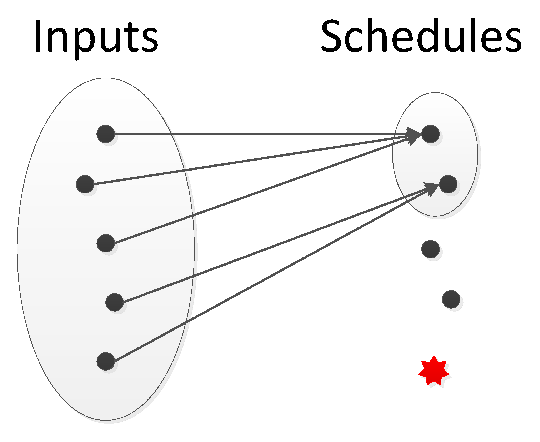
\includegraphics[width=.5\linewidth]{figures/smt}
%% \caption{\em Stable (deterministic) multithreading.} \label{fig:smt}
%% \end{figure}

Second, the overhead of enforcing a schedule on different inputs is low.
Presumably, the exponentially many schedules allow the
runtime system to react to various timing factors and select an
efficient schedule.  However, results from the \smt systems we built
invalidated this presumption.  With carefully designed schedule
representations (\S\ref{sec:relax}), our systems incurred less than 15\%
overhead enforcing schedules on different inputs for most evaluated programs
(\S\ref{sec:eval}).  We believe this moderate overhead is worth the gains
in reliability.
% In general, users most likely prefer a slightly slower
% program that computes correct results than a faster program that
% frequently crashes.

Leveraging these insights, we have invented \emph{stable multithreading
  (\smt)}, a new multithreading approach that reuses each schedule on a wide
range of inputs, mapping all inputs to a dramatically reduced set of schedules.
By vastly shrinking the haystack, it addresses all the needle-in-a-haystack
challenges at once.  In addition, \smt stabilizes program behaviors
on inputs that map to the same schedule and minor program changes that
do not affect the schedules, providing robustness and stability
anticipated by developers and users.

\smt and DMT are orthogonal. \smt aims to reduce the set of schedules for
\emph{all} inputs, whereas DMT aims to reduce the schedules for \emph{each} input (down
to one).  A \smt system may be either deterministic or nondeterministic.
Figure~\ref{fig:smt} and Figure~\ref{fig:smtn} depict two \smt systems: the
many-to-one mapping in Figure~\ref{fig:smt} is deterministic, while the
many-to-few mapping in Figure~\ref{fig:smtn} is nondeterministic.  A
many-to-few mapping improves performance because the
runtime system can choose an efficient schedule out of a few for an input
based on current timing factors, but it increases the efforts and
resources needed for reliability.  Fortunately, the choices of schedules
are only a few (\eg, a small constant such as two), so the challenges
caused by nondeterminism are easy to solve.

%% \begin{figure}[t]
%% \centering
%% 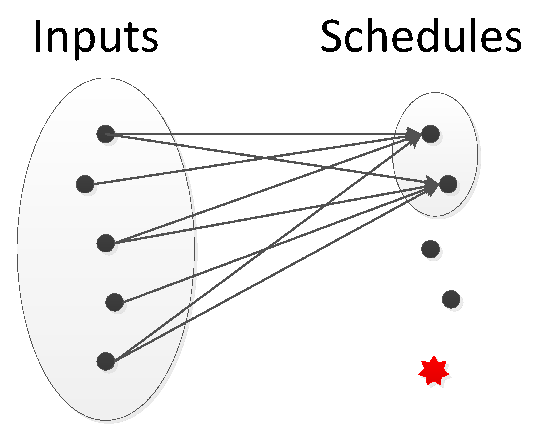
\includegraphics[width=.5\linewidth]{figures/smtn}
%% \caption{\em Stable (nondeterministic) multithreading.} \label{fig:smtn}
%% \end{figure}

%% The \smt mapping in Figure~\ref{fig:smt} is also deterministic because it
%% maps an input to only one schedule.  However, \smt need not be
%% deterministic; Figure~\ref{fig:smtn} depicts a \smt mapping
%% that maps many inputs to a few schedules.  
%% Having a few choices of schedules improves performance: the system can
%% process an input by choosing one out of the few schedules based on
%% current timing factors.  Although this many-to-few mapping is nondeterministic,
%% the choices of schedules are only a few (\eg, a small constant), so the
%% problems caused by nondeterminism does not exist here.  For instance, to
%% reproduce a bug, developers can afford to retry a few schedules.
%% Furthermore, the overall number of schedules remains small, so the same
%% advantages of \smt apply.

%% runtime system chooses one from a few schedules to process an input.
%% non-deterministic, but because the possibility.
%% nondeterministic is okay! if total number of schedules is small.
%% a few more choices, react better to scheduling.

%% special case: many-to-one, both stable and deterministic.

%% enforces a $m:c$ mapping where $c$ is a small constant.  If $c$ is 1, then
%% the system is both stable and deterministic.
%% and Figure~\ref{fig:stable-det} illustrate

%% both a general stable multithreading system and a stable and deterministic
%% multithreading system.

%% represents a schedule as a synchronization order because a
%% synchronization order can be efficiently enforced.  An additional
%% advantage of the synchronization order representation is that it can be
%% frequently reused.  The intuition is that synchronizations map to
%% developer intents of inter-thread control flows.  By enforcing the same
%% synchronization order, we enforce the same inter-thread ``path'', but do
%% not restrict what data can flow down this path.  Just like a sequential
%% path can process many different inputs observed in profiling
%% work~\cite{fisher:branch:asplos92,ball:branch:pldi93,ball:path:micro29}, an
%% inter-thread ``path'' can also process many different inputs.

%% schedule-centric

%% Our plan to address the aforementioned reliability challenges is to
%% drastically reduce the number of schedules.  To do so, our insight is that
%% we can frequently reuse one schedule to process a wide range of inputs.
%% The reason is that a schedule fixes only the communication aspect of an
%% execution, but it allows flexible local computations that do not affect
%% the communication.  For instance, consider a parallel compression utility
%% \pbzip that splits a file into multiple blocks and compresses these blocks
%% in parallel using multiple threads.  Empirically, we found that many
%% programs we studied can frequently reuse schedules.  For instance, Apache
%% 90\%.  Table~\ref{tab:reuse-rate}. FFT. bitonic sort.
    
%% We therefore propose a new approach to multithreading called \emph{stable
%%   multithreading (\smt)} that forces a multithreaded program to reuse
%% schedules if possible, even over different inputs.  In contrast to the
%% $1:1$ mapping between inputs and schedules enforced by a DMT system, a \smt
%% system essentially enforces a $m:c$ mapping where $c$ is a small constant.
%% If $c$ is 1, then the system is both stable and deterministic.
%% Figure~\ref{fig:stable-not-det} and Figure~\ref{fig:stable-det} illustrate
%% both a general stable multithreading system and a stable and deterministic
%% multithreading system.

% usage scenarios.

%% In retrospect, the \smt approach is almost obvious.  Consider a non-tech
%% analogy.  A multithreaded execution is like a group of cars driving down
%% parallel lanes, where the group of cars is the input and the sequence of
%% lane changes (``lane-change plan'') is the schedule.  A buggy schedule
%% causes a program to misbehave, like an unsafe lane-change plan causing
%% cars to collide.  Determinism guarantees that each group of cars sticks to
%% one lane-change plan, but given enough groups of cars and an arbitrary
%% plan for each group, some group will eventually collide.  In contrast, \smt
%% focuses on reducing the plans.  If there is already a plan for a group of
%% cars to safely change lanes, why don't we also stick to the plan for the
%% other groups of cars?  By doing so, we not only avoid unknown plans that
%% may lead to collisions, but also amortize the cost of making the plan and
%% setting up lane dividers.


%% In retrospect, the \smt approach is almost obvious.  Recall our non-tech analogy of
%% cars driving down parallel lanes.  If there is already a plan for a group
%% of cars to safely change lanes, why don't we also stick to the plan for
%% the other groups of cars?  By doing so, we not only avoid unknown plans
%% that may lead to collisions, but also amortize the cost of making the
%% plan and setting up lane dividers.

\subsection{Benefits}

By vastly reducing the set of schedules, \smt brings numerous reliability benefits
to multithreading.  We describe several:

\para{Testing.} \smt automatically
increases the coverage of schedule testing tools, with coverage
defined as the ratio of tested schedules over all schedules.
For instance, consider \pbzip again which needs only two
schedules for each different number of threads under typical setups.  Testing 32 schedules effectively covers from
1 to 16 threads.  Given that (1) \pbzip achieves peak performance when the
number of threads is identical or close to the number of cores
and (2) a typical machine has up to 16 cores, 32 tested schedules can
practically cover most schedules executed in the field.

\para{Debugging.} Reproducing a bug now does not require the exact input,
as long as the original and the altered inputs map to the same schedule.
It does not require the exact program either, as long as the changes to
the program do not affect the schedule.  Users may remove private
information such as credit card numbers from their bug reports. Developers
may reproduce the bugs in different environments or add \v{printf}
statements.

\para{Analyzing and verifying programs.} Static analysis can now focus
only on the set of schedules enforced in the field, gaining
precision.  Dynamic analysis enjoys the same benefits as testing.  Model
checking can now check drastically fewer schedules, mitigating the so-called
``state explosion'' problem~\cite{clarke:ModelChecking}.  Interactive theorem proving becomes easier, too,
because verifiers need to prove theorems only on the set of schedules
enforced in the field.  We will describe these benefits in more detail in
\S\ref{sec:specialize}.

\para{Avoiding errors at runtime.}  Programs can also adaptively learn correct
schedules in the field, then reuse them on future inputs to avoid unknown,
potentially buggy schedules.  We will describe this benefit in more
detail in \S\ref{sec:memoize}.

\subsection{Caveats}

\smt is certainly not for every multithreaded program.  It works well with
programs whose schedules are loosely coupled with inputs,
%, in particular, programs that divide computation based on static factors such as the number of cores.
but there are also other programs.  For instance, a program may decide to spawn
%% a program may not be able to
%% divide computation upfront; instead, it has to dynamically balance the
%% load as the program runs.  Similarly,
threads or invoke synchronizations based on intricate conditions involving many bits in the input.
The parallel \v{grep}-like utility \pfscan is an example.  It searches for a
keyword in a set of files using multiple threads, and for each match, it
grabs a lock to increment a counter.  A schedule computed on one set of
files is unlikely to suit another.
To increase the input range each schedule covers, developers can
exclude the operations on this lock from the schedule using annotations.


\smt provides robustness and stability on small input and program
perturbations when they do not affect schedules.  However, there
is still room to improve.  For instance, when developers change their
programs by adding synchronizations, it may be more efficient to
update previously computed schedules rather than to recompute from
scratch. We leave this idea for future work.
